\documentclass{fast_latex}

\usepackage{inputenc}
\usepackage{lastpage}
\usepackage{setspace}
\usepackage{graphicx}
\usepackage[pdfborder={0 0 0}]{hyperref}		% turn on when latex is used (not miktec)
\usepackage{url} % LEO: urls \url{}
\usepackage{verbatim} % code and comment
\usepackage{longtable}
\usepackage{xspace}   % whitespace after a macro if no punctuation after the macro
\usepackage{multirow}
\usepackage{colortbl}
\usepackage{longtable}
\usepackage{array}
\usepackage{amssymb}
\parindent0pt


\newcommand\deliverableNumber{D5.2.1}
\newcommand\deliverableTitle{Prototype Semantic Catalogue for Screen-Flow Gadgets and Back-End Services}
\newcommand\deliverableTitleShort{Prototype Semantic Catalogue}
\newcommand\workpackageNumber{5}
\newcommand\workpackageTitle{Semantic catalogue of screen-flow resources and back-end Web Services}
\newcommand\authorOne{Ismael Rivera, NUIG}
\newcommand\authorTwo{Author 2}
\newcommand\authorThree{Author 3}
\newcommand\authorFour{Author 4}

\begin{document}
% explicit hyphenations
\hyphenation{RDF-Re-po-si-to-ry}
\hyphenation{name-space}

%\fontfamily{tahoma}\selectfont
\def\note#1{\marginpar{\footnotesize#1}} % use this to show the notes in the document
%\def\note#1{} % use this to hide the notes


\newenvironment{definition}{}{}

%%%%%%%%%%%%%%%%%%%%%%%%%%%%%%%%%%%%%%%%%%%%%%%%%%%%%%%%%%%%%%%%%%%%%%%%%%%%%%%%
% TITLE PAGES 
%%%%%%%%%%%%%%%%%%%%%%%%%%%%%%%%%%%%%%%%%%%%%%%%%%%%%%%%%%%%%%%%%%%%%%%%%%%%%%%%
\thispagestyle{empty}

\pagenumbering{roman}

\begin{flushright}
	
\includegraphics[width=3cm]{images/FP7_logo}
\end{flushright}

\vspace{1cm}

%\begin{minipage}[p]{15cm}
	\begin{center}
		
\includegraphics{images/FAST_logo}\\
		\vspace{1cm}
		{\LARGE{\sffamily \emph{FAST AND ADVANCED STORYBOARD TOOLS}}}\\
		\vspace{0.5cm}
		{\LARGE \sffamily \emph{FP7-ICT-2007-1-216048}}\\
		\vspace{0.5cm}
		{\LARGE \sffamily \emph{http://fast.morfeo-project.eu}}\\
		\vspace{4cm}
		{\LARGE \sffamily \textbf{Deliverable \deliverableNumber}}\\
		\vspace{0.5cm}
		{\LARGE \sffamily \textbf{\deliverableTitle}}\\
		\vspace{2cm}
		{\large \sffamily \authorOne}\\
		\vspace{0.5cm}
		\vfill
		{\large \sffamily Date: 20/02/2009}\\
		\vspace{1cm}
		{\sffamily FAST is partially funded by the E.C. (grant code: FP7-ICT-2007-1-216048).}
		
	\end{center}
%\end{minipage}


\clearpage
%%%%%%%%%%%%%%
% NEXT PAGES %
%%%%%%%%%%%%%%
\pagestyle{scrheadings}

\lohead{
\includegraphics[width=4cm]{images/FAST_logo_transparent}}
%\cohead{\small\textcolor{fast@lightgrey}{\deliverableTitle}}
\rohead{\small{\today}}
%\lofoot{\small\textcolor{fast@lightgrey}{Task Force Ontologies}}
\cofoot{\small{FAST 216048 --- \deliverableTitleShort}}
\rofoot{\small{\thepage}}

\newpage

\clearpage

\section*{Version History}

\begin{small}
\begin{tabular}{|l|l|l|p{7.5cm}|}
\hline
\rowcolor{fast@lightgrey}\textcolor{white}{\textbf{Rev. No.}} &
                         \textcolor{white}{\textbf{Date}} &
                         \textcolor{white}{\textbf{Author (Partner)}} &
                         \textcolor{white}{\textbf{Change description}}\\ \hline
1.0 & 20/02/2009 & Ismael Rivera (NUIG) & First version of the deliverable \\ \hline
\end{tabular}
\end{small}

\color{black}

\vfill
%{\bf Explanations of abbreviations on front page}\\
%\\
%%Nature \\
%R: Report \\
%P: Prototype \\
%R/P: Report and Prototype \\
%O: Other \\
% \\
%Dissemination level \\
%PU: Public \\
%PP: Restricted to other FP6 participants \\
%RE: Restricted to specified group \\
%CO: Confidential, only for NEPOMUK partners \\

\newpage

%%%%%%%%%%%%%%%%%%%%%
% Executive Summary %
%%%%%%%%%%%%%%%%%%%%%

\clearpage

\section*{Executive Summary}
\doublespacing

The present deliverable is intented to be the developer's manual of the prototype of the semantic catalogue. That said, whoever developing a component which will interact with the catalogue will find in this document a description of its architecture, the functionality provided together with the API (Application Programming Interface), data interchange formats, code errors and exceptions as well as several examples of usage.

\newpage

%%%%%%%%%%%%%%%%%%%%%
% Document Summary %
%%%%%%%%%%%%%%%%%%%%%

\clearpage

\section*{Document Summary}
% double spacing from here on:
\singlespacing

\begin{small}
\begin{tabular}
	%{| >{\columncolor{fast@lightgrey}}p{3.25cm}|p{6cm}|p{2cm}|p{2cm}|}
	{| >{\columncolor{fast@lightgrey}}p{3.25cm}|p{6cm}|p{2cm}|p{2cm}|}
	\hline
	\textcolor{white}{\textbf{Code}} & {FP7-ICT-2007-1-216048} & {\textbf{Acronym}} & {FAST}\\ \hline
	\textcolor{white}{\textbf{Full title}} & \multicolumn{3}{l|}{Fast and Advanced Storyboard Tools}\\ \hline
	\textcolor{white}{\textbf{URL}} & \multicolumn{3}{l|}{\url{http://fast.morfeo-project.eu}}\\ \hline
	\textcolor{white}{\textbf{Project officer}} & \multicolumn{3}{l|}{Annalisa Bogliolo}\\ \hline
\end{tabular}
\end{small}

\vspace{0.5cm}

\begin{small}
\begin{tabular}
	{| >{\columncolor{fast@lightgrey}}p{3.25cm}|p{1.25cm}|p{1cm}|p{1cm}|p{6.32cm}|}
	\hline
	\textcolor{white}{\textbf{Deliverable}} & {\textbf{Number}} & {\deliverableNumber} & {\textbf{Name}} & {\deliverableTitle}\\ \hline
	\textcolor{white}{\textbf{Work package}} & {\textbf{Number}} & {\workpackageNumber} & {\textbf{Name}} & {\workpackageTitle}\\ \hline
\end{tabular}
\end{small}

\vspace{0.5cm}

\begin{small}
\begin{tabular}
	{| >{\columncolor{fast@lightgrey}}p{3.25cm}|p{1.4cm}|p{3.28cm}|p{1.6cm}|p{3.29cm}|}
	\hline
	\textcolor{white}{\textbf{Delivery data}} & {\textbf{Due date}} & {27/02/2009} & {\textbf{Submitted}} & {27/02/2009}\\ \hline
	\textcolor{white}{\textbf{Status}} & \multicolumn{2}{l|}{Status} & \multicolumn{2}{l|}{final}\\ \hline
	\textcolor{white}{\textbf{Dissemination Level}} & \multicolumn{4}{l|}{Public $\boxtimes$ / Consortium $\square$}\\ \hline
	\textcolor{white}{\textbf{Short description of contents}} & \multicolumn{4}{p{10.85cm}|}{This deliverable is the technical documentation for the prototype developed as part of the WP5. It describes the catalogue's architecture, data interchange formats, APIs and examples of how to interact with it.}\\ \hline
	\textcolor{white}{\textbf{Authors}} & \multicolumn{4}{l|}{\authorOne}\\
%	{} & \multicolumn{4}{l|}{\authorOne}\\ 
%	{} & \multicolumn{4}{l|}{\authorOne}\\ 
%	{} & \multicolumn{4}{l|}{\authorOne}\\
  \hline
	\textcolor{white}{\textbf{Deliverable Owner}} & \multicolumn{2}{l|}{\authorOne} & \textbf{email} & {ismael.rivera@deri.org} \\ \cline{4-5}
	\textcolor{white}{\textbf{(Partner)}} & \multicolumn{2}{l|}{} & \textbf{phone} & {+353 91 495086} \\ \hline
	\textcolor{white}{\textbf{Keywords}} & \multicolumn{4}{p{10.85cm}|}{FAST, semantic catalogue, gadget catalogue, RDF store}\\ \hline
\end{tabular}
\end{small}

\newpage

%%%%%%%%%%%%%%%%%%%%%
% TABLE OF CONTENTS %
%%%%%%%%%%%%%%%%%%%%%
\doublespacing
\setcounter{tocdepth}{2}
\tableofcontents
\cleardoublepage
\pagenumbering{arabic}


%%%%%%%%%%%%%%%%%%%%%%%%%
% BEGINNING OF SECTIONS %
%%%%%%%%%%%%%%%%%%%%%%%%%
\rofoot{\small{Page \thepage\ of \pageref{LastPage}}} 

\clearpage
\section{Introduction}
\label{sec:introduction}
This section starts establishing the goal and scope of the present document, shows how it is structured and details the relation to others documents and work packages.

\subsection{Goal and Scope}
This is an introductory manual for developers who want to adopt and use the FAST semantic catalogue. It explains the main functionalities implemented so far, an overview of its architecture and a detailed \emph{Application Programming Interface} or API of the complete set of the operations offered through a REST service.

\subsection{Structure of the document}
The deliverable presents both the external and internal architecture in Section \ref{sec:architecture}, then in Section \ref{sec:api} it is detailed the Catalogue API, query formats, interchange formats, error codes and so on, and the document ends by stating some conclusions and future directions of the semantic catalogue in Section \ref{sec:conclusions}.

\subsection{Overall approach for WP5 and relation to other Work Packages and Deliverables}
The main objective of the Work Package 5, as specified in \cite{DoW}, includes the development of the FAST semantic catalogue, considered the back-end of the FAST platform, which will store and index any kind of resources such as screen-flows, screens, back-end Web services descriptions, locate appropriate gadgets, resources and Web services for users, storing and indexing user profiles, and resolve mediation problems between gadgets, back-end services and the different ontologies stored.

The deliverables stated in \cite{DoW} for this WP are:
\begin{description}
	\item[User manual of the FAST Catalogue] This is the user manual of the catalogue, but is out of scope in this iteration of the project.
	\item[Prototype semantic catalogue for screen-flow gadgets and back-end services] This deliverable is a software prototype of the semantic catalogue for experimentation purposes. Apart from the software, it will be created technical documentation and manuals for developers as the present document.
\end{description}

The semantic catalogue relies strongly on the FAST ontology defined in \cite{moeller2009fast_ontology} since the ontology defines how every element within FAST will be internally stored by the catalogue, and takes into consideration specific requirements detailed in \cite{fast_requirements} where the functionalities of the complete FAST tool are defined.


\clearpage
\section{Architecture}
\label{sec:architecture}
This section details the internal catalogue's architecture and which external components will interact with it. Basically three layers can be distinguished: Presentation, Business Logic and Persistence layer (see Figure \ref{fig:architecture}). 

\begin{figure}[htb]
\label{fig:architecture}
\begin{center}
	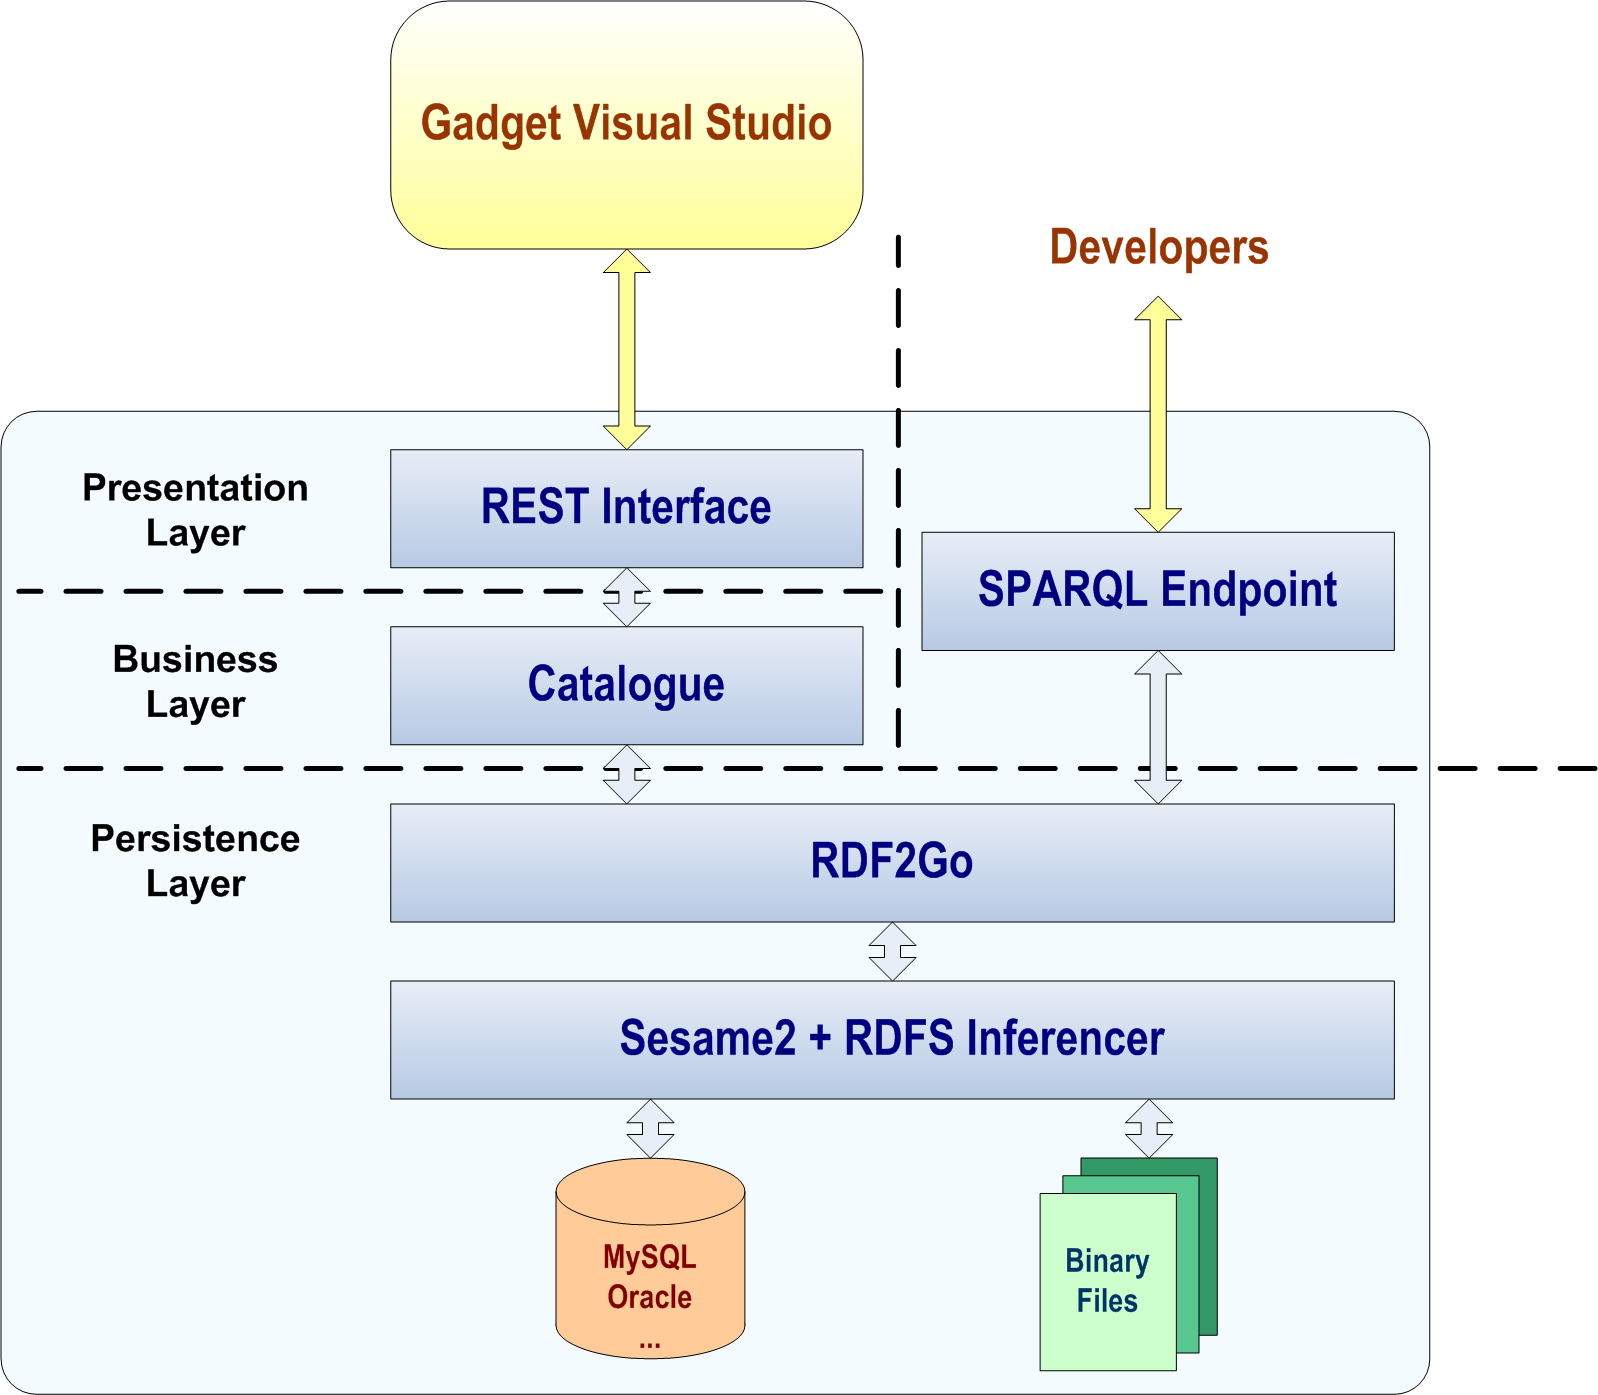
\includegraphics[width=12cm]{images/catalogue_architecture}
	\caption{Catalogue's Architecture}
	\label{fig:CatalogueInternalArchitecture}
\end{center}
\end{figure}

The Presentation layer will be the public interface of the catalogue. The main purpose of this layer is to provide its functionality to other components within the Gadget Visual Studio. The service is offered in a REST (REpresentational State Transfer) style, making it easy to consume than other complex APIs. REST is an architectural style, not a toolkit or a standard. Even though, it makes use of standards like HTTP, URI, Resource Representations (XML, HTML, JSON, JPEG, etc.) or MIME types (text/xml, text/html, application/json, image/jpeg, etc.). Another characteristic of the REST style is its stateless assumption. The catalogue adopts this strategy; therefore every request needs a complete set of information in order to prepare the response.

As part of the Presentation layer, a SPARQL endpoint is offered using the SPARQL protocol service as defined in the SPROT \cite{sprot} specification. The SPARQL endpoint is mostly offered to enable other developers to query directly the catalogue knowledge base using SPARQL queries. This feature is supported by the Sesame RESTful HTTP interface for SPARQL Protocol for RDF.

The Business Logic layer contains all the FAST domain-specific processing. It provides functions to interact with all the elements of the domain model specified in \cite{moeller2009fast_ontology}. It processes the input from the Presentation layer, creating specific objects modelling the business logic, and vice versa. In addition it interacts with the Persistence layer in order to persist the model.

The Persistence layer provides an API which allows the Business layer to work with a standard set of objects that read and save their state to the triple store. For this reason, on top of this layer it is used RDF2Go, an abstraction over triple (and quad) stores. The RDF2Go API allows interacting with the semantic representation of the model (triples) in a generic manner, and also brings the flexibility of choosing different triple stores to persist them. The selected implementation for the triple stored is Sesame 2. Moreover, this framework is completely extensible and configurable regarding to storage mechanisms, inferencers, RDF file formats, query result formats and query languages. For the actual catalogue prototype, the storage mechanism used is the native file storage system of Sesame, the inferencer used is a subset of the RDFS entailment rules \cite{rdfsrules} following a forward-chaining policy. 



\clearpage
\section{RESTful Catalogue API}
\label{sec:api}
This section provides a high-level overview of the Catalogue API. It describes the calls or operations supported, specific parameters and responses for each operation, supported interchange formats and some examples to facilitate the understanding of the API.


\subsection{JSON Interchange Format}
The format supported by the Catalogue API for all the request and responses is JSON\footnote{http://www.json.org/}. JSON is a lightweight data interchange format whose simplicity has resulted in widespread use among web developers, easy to read and write and able to using any programming language because its structures map directly to data structures used in most programming languages.

Every HTTP request and response is encoded using the MIME type \texttt{application/json} and the charset \texttt{UTF-8}.

\subsubsection{Example of a screen}
\begin{verbatim}
{
  "uri": null,
  "label": {"en-GB": "Screen - DERI"},
  "description": {"en-GB": "Returns people working in DERI"},
  "creationDate": "2009-02-07T09:59:52+0000",
  "creator": "http://www.ismaelrivera.es/",
    "domainContext": {
      "tags": [],
      "user": null
    },
  "homepage": "http://www.deri.ie/",
  "icon": "http://www.deri.ie/icon.jpg",
  "screenshot": "http://www.deri.ie/screenshot.jpg",
  "rights": "http://creativecommons.org/",
  "version": "1.0",
  "preconditions": [],
  "postconditions": ["?person rdf:type foaf:Person . 
                      ?person foaf:workplaceHomepage http://www.deri.ie/"]
}
\end{verbatim}

\subsubsection{Internationalisation I18n}
In order to offers an adaptable solution to various languages and regions without major engineering changes, internationalisation is considered from an early stage in the catalogue development. Underlying representation technologies used to develop the catalogue (RDF and JSON) allow to implement this feature. This feature is implemented by the addition of a language tag to every 'string' desired. The specification of this language tag is composed by the language code and the country code, following the ISO 639\footnote{http://ftp.ics.uci.edu/pub/ietf/http/related/iso639.txt} for languages and the ISO 3166\footnote{http://userpage.chemie.fu-berlin.de/diverse/doc/ISO\_3166.html} for countries. The following example illustrates how to use it properly in both formats.

\begin{verbatim}
{
  "label": {
    "en-GB": "Simple Example",
    "es-ES": "Ejemplo Sencillo",
    "de-DE": "Einfaches Beispiel"
  },
  "description": {
    "en-GB": "This is a simple example of a screen",
    "es-ES": "Esto es un ejemplo sencillo de pantalla",
    "de-DE": "Dies ist ein einfaches Beispiel f�r einen Bildschirm"
  },
}
\end{verbatim}

\begin{verbatim}
<rdf:Description rdf:about="http://www.morfeoproject.eu/fast/fco#ExampleScreen">
  <rdf:type rdf:resource="http://www.morfeoproject.eu/fast/fco#Screen"/>
  <rdfs:label xml:lang="en-GB">Simple Example</rdfs:label>
  <rdfs:label xml:lang="es-ES">Ejemplo Sencillo</rdfs:label>
  <rdfs:label xml:lang="de-DE">Einfaches Beispiel</rdfs:label>
  <description
    xmlns="http://purl.org/dc/terms/"
    xml:lang="en-GB">This is a simple example of a screen</description>
  <description
    xmlns="http://purl.org/dc/terms/"
    xml:lang="es-ES">Esto es un ejemplo sencillo de pantalla</description>
  <description
    xmlns="http://purl.org/dc/terms/"
    xml:lang="de-DE">Dies ist ein einfaches Beispiel f�r einen Bildschirm</description>
</rdf:Description>
\end{verbatim}

By now it is allowed using internationalisation for the label and the description of a screen, but more attributes will be benefited by this feature.


\subsection{API Calls}
This section contains detailed descriptions of the interface provided by the catalogue via REST services, detailing request parameters, response elements, any special errors and examples of requests and responses. The URL format is also specified for each operation, where 'catalogueURL' has to be replaced for the real URL the service is installed (e.g. forge.morfeo-project.org/catalogue).

\subsubsection{CRUD operations for Screens}
A screen is a resource which can be created, retrieved, modified or deleted since the catalogue provides CRUD support for screens. These features are provided following the REST philosophy, using the HTTP methods. Two concepts have to be defined: \emph{collection}, as a set of screens which access URI is http://catalogueURL/screens/ where catalogueURL is the specific URL where the catalogue server is installed, and \emph{member} of the collection, in other words, the screen itself, which access URI is http://catalogueURL/screens/<id> where the <id> has to be replaced by the identifier of a screen. The details of the operations and which HTTP verb has to be used can be found in the Table \ref{tab:crud_screens}.

\begin{table}[htb]
\caption{CRUD operations for Screens}
\label{tab:crud_screens}
\begin{center}
\begin{tabular}{|p{2.5cm}|p{2.5cm}|p{3.5cm}|p{5cm}|}
\hline
\rowcolor{fast@lightgrey}\textcolor{white}{Resource} &
                         \textcolor{white}{HTTP method} &
                         \textcolor{white}{HTTP body} &
                         \textcolor{white}{Description}\\ \hline
Collection URI & GET & N/A & \textbf{List} the members of the collection.\\ \hline
Collection URI & PUT & N/A & Not used.\\ \hline
Collection URI & POST & JSON representation of the screen & \textbf{Create} a new entry in the collection where the URI is assigned automatically by the collection. The URI created is returned by this operation.\\ \hline
Collection URI & DELETE & N/A & Not used.\\ \hline
Member URI & GET & N/A & \textbf{Retrieve} the addressed member of the collection.\\ \hline
Member URI & PUT & JSON representation of the screen & \textbf{Update} the addressed member of the collection or create it with a defined URI.\\ \hline
Member URI & POST & N/A & Not used. \\ \hline
Member URI & DELETE & N/A & \textbf{Delete} the addressed member of the collection.\\ \hline
\end{tabular}
\end{center}
\end{table}

Here are shown various examples of request and responses using the catalogue server. To create a new screen, a POST request is send to the catalogue server, including the JSON representation of the screen as the body of the request:

\begin{verbatim}
{
  "uri": null,
  "label": {"en-GB": "Screen - DERI"},
  "description": {"en-GB": "Returns people working in DERI"},
  "creationDate": "2009-02-07T09:59:52+0000",
  "creator": "http://www.ismaelrivera.es/",
    "domainContext": {
      "tags": [],
      "user": null
    },
  "homepage": "http://www.deri.ie/",
  "icon": "http://www.deri.ie/icon.jpg",
  "screenshot": "http://www.deri.ie/screenshot.jpg",
  "rights": "http://creativecommons.org/",
  "version": "1.0",
  "preconditions": [],
  "postconditions": ["?person rdf:type foaf:Person . 
                      ?person foaf:workplaceHomepage http://www.deri.ie/"]
}
\end{verbatim}

The URI will be not taken into account since the catalogue will generate a unique URI for each resource created. So, the response for this operation is:

\begin{verbatim}
{
  "creationDate": "2009-02-07T09:59:52+0000",
  "creator": "http://www.ismaelrivera.es/",
  "description": {"en-GB": "Show information about a person working in DERI"},
  "domainContext": {
    "tags": [],
    "user": "null"
  },
  "homepage": "http://www.deri.ie/",
  "icon": "http://www.deri.ie/icon.jpg",
  "label": {"en-GB": "Screen - DERI"},
  "postconditions": [],
  "preconditions": ["?person rdf:type foaf:Person . 
                     ?person foaf:workplaceHomepage http://www.deri.ie/"],
  "rights": "http://creativecommons.org/",
  "screenshot": "http://www.deri.ie/screenshot.jpg",
  "uri": "http://www.morfeoproject.eu/fast/fco#Screen1234552194269",
  "version": "1.0"
}
\end{verbatim}

To obtain all the screens stored in the catalogue a HTTP GET request is sent to the Collection URI and the response may be something like this:
\begin{verbatim}
[
  {
    "creationDate": "2009-02-07T09:59:52+0000",
    "creator": "http://www.ismaelrivera.es/",
    "description": {"en-gb": "Returns people working in DERI"},
    "domainContext": {
      "tags": [],
      "user": null
    },
    "homepage": "http://www.deri.ie/",
    "icon": "http://www.deri.ie/icon.jpg",
    "label": {"en-gb": "Screen - DERI"},
    "postconditions": ["?person rdf:type foaf:Person . 
                        ?person foaf:workplaceHomepage http://www.deri.ie/"],
    "preconditions": [],
    "rights": "http://creativecommons.org/",
    "screenshot": "http://www.deri.ie/screenshot.jpg",
    "uri": "http://www.morfeoproject.eu/fast/fco#Screen1234552164472",
    "version": "1.0"
  },
  {
    "creationDate": "2009-02-07T09:59:52+0000",
    "creator": "http://www.ismaelrivera.es/",
    "description": {"en-gb": "Show information about a person working in DERI"},
    "domainContext": {
      "tags": [],
      "user": null
    },
    "homepage": "http://www.deri.ie/",
    "icon": "http://www.deri.ie/icon.jpg",
    "label": {"en-gb": "Screen - DERI"},
    "postconditions": [],
    "preconditions": ["?person rdf:type foaf:Person . 
                       ?person foaf:workplaceHomepage http://www.deri.ie/"],
    "rights": "http://creativecommons.org/",
    "screenshot": "http://www.deri.ie/screenshot.jpg",
    "uri": "http://www.morfeoproject.eu/fast/fco#Screen1234552194269",
    "version": "1.0"
  },
  {
    "creationDate": "2009-02-07T09:59:52+0000",
    "creator": "http://www.ismaelrivera.es/",
    "description": {"en-gb": "Show information about a person"},
    "domainContext": {
      "tags": [],
      "user": null
    },
    "homepage": "http://www.deri.ie/",
    "icon": "http://www.deri.ie/icon.jpg",
    "label": {"en-gb": "Screen - DERI"},
    "postconditions": [],
    "preconditions": ["?person rdf:type foaf:Person"],
    "rights": "http://creativecommons.org/",
    "screenshot": "http://www.deri.ie/screenshot.jpg",
    "uri": "http://www.morfeoproject.eu/fast/fco#Screen1234552373865",
    "version": "1.0"
  }
]
\end{verbatim}


\subsubsection{CRUD operations for Screen-Flows}
A screenflow is a resource which can be created, retrieved, modified or deleted since the catalogue provides CRUD support for screenflows. These features are provided following the REST philosophy, using the HTTP methods. As in the previous section the concepts \emph{collection} and \emph{member} are used including their URLs. Table \ref{tab:crud_screenflows} details the operations offered for screen-flows.

\begin{table}[htb]
\caption{CRUD operations for Screen-Flows}
\label{tab:crud_screenflows}
\begin{center}
\begin{tabular}{|p{2.5cm}|p{2.5cm}|p{3.5cm}|p{5cm}|}
\hline
\rowcolor{fast@lightgrey}\textcolor{white}{Resource} &
                         \textcolor{white}{HTTP method} &
                         \textcolor{white}{HTTP body} &
                         \textcolor{white}{Description}\\ \hline
Collection URI & GET & N/A & \textbf{List} the members of the collection.\\ \hline
Collection URI & PUT & N/A & Not used.\\ \hline
Collection URI & POST & JSON representation of the screen-flow & \textbf{Create} a new entry in the collection where the URI is assigned automatically by the collection. The URI created is returned by this operation.\\ \hline
Collection URI & DELETE & N/A & Not used.\\ \hline
Member URI & GET & N/A & \textbf{Retrieve} the addressed member of the collection.\\ \hline
Member URI & PUT & JSON representation of the screen-flow & \textbf{Update} the addressed member of the collection or create it with a defined URI.\\ \hline
Member URI & POST & N/A & Not used. \\ \hline
Member URI & DELETE & N/A & \textbf{Delete} the addressed member of the collection.\\ \hline
\end{tabular}
\end{center}
\end{table}

The following is an example of the request and response while creating a screen-flow:
\begin{verbatim}
{
  "uri": null,
  "label": {"en-GB": "My First ScreenFlow"},
  "description": {"en-GB": "A example of screenflow"},
  "creationDate": "2009-02-05T13:11:41+0000",
  "creator": "http://www.ismaelrivera.es/",
  "domainContext": {
    "tags": ["people"],
    "user": null
  },
  "homepage": "http://www.screenflow.com/",
  "icon": "http://www.screenflow.com/icon.jpg",
  "screenshot": "http://www.screenflow.com/screenshot.jpg",
  "rights": "http://creativecommons.org/",
  "version": "1.0",
  "preconditions": [],
  "postconditions": [],
  "screens": [
    "http://www.morfeoproject.eu/fast/fco#Screen1233750841383",
    "http://www.morfeoproject.eu/fast/fco#Screen1233750828836",
    "http://www.morfeoproject.eu/fast/fco#Screen1233750820914"
  ]
}
\end{verbatim}

\begin{verbatim}
{
  "creationDate": "2009-02-05T13:11:41+0000",
  "creator": "http://www.ismaelrivera.es/",
  "description": {"en-GB": "A example of screenflow"},
  "domainContext": {
    "tags": ["people"],
    "user": null
  },
  "homepage": "http://www.screenflow.com/",
  "icon": "http://www.screenflow.com/icon.jpg",
  "label": {"en-GB": "My First ScreenFlow"},
  "postconditions": [],
  "preconditions": [],
  "rights": "http://creativecommons.org/",
  "screens": [
    "http://www.morfeoproject.eu/fast/fco#Screen1233750841383",
    "http://www.morfeoproject.eu/fast/fco#Screen1233750828836",
    "http://www.morfeoproject.eu/fast/fco#Screen1233750820914"
  ],
  "screenshot": "http://www.screenflow.com/screenshot.jpg",
  "uri": "http://www.morfeoproject.eu/fast/fco#ScreenFlow1233752391898",
  "version": "1.0"
}
\end{verbatim}


\subsubsection{Find}
The find operation search inside the catalogue for any screen which could be somehow related to the gadget the user is creating. It provides a recommended set of screens depending on the domain context, the canvas, etc. The specific URL to access this operation is http://catalogueURL/find using HTTP POST method. From now on, the method 'find' only considers the domain context, being a list of tags and the pre/postconditions of the screens. It will try to satisfy all the unsatisfied preconditions of a given list of screens also known as canvas. The results will be all the screens stored in the catalogue which fulfil some of these preconditions, and are tagged with the tags specified in the domain context. The request parameters are shown in Table \ref{tab:find_request} and the response parameters are shown in Table \ref{tab:find_response}.

\begin{table}[htb]
\caption{Find Request Parameters}
\label{tab:find_request}
\begin{center}
\begin{tabular}{|p{2cm}|p{9.5cm}|p{2cm}|}
\hline
\rowcolor{fast@lightgrey}\textcolor{white}{Name} &
                         \textcolor{white}{Description} &
                         \textcolor{white}{Type}\\ \hline
Canvas & The canvas is composed by a list of screens. Only the URI is needed. & Optional \\ \hline
Domain Context & The domain context contains a list of tags and a user. & Optional \\ \hline
Elements & It is a list of resources, previously stored in the catalogue. For example, the list of screens recommended last execution. Only accepts screens. & Optional \\ \hline
\end{tabular}
\end{center}
\end{table}

\begin{table}[htb]
\caption{Find Response Parameters}
\label{tab:find_response}
\begin{center}
\begin{tabular}{|p{2cm}|p{9.5cm}|p{2cm}|}
\hline
\rowcolor{fast@lightgrey}\textcolor{white}{Name} &
                         \textcolor{white}{Description} &
                         \textcolor{white}{Type}\\ \hline
N/A & A list of recommended screens is returned. & Required \\ \hline
\end{tabular}
\end{center}
\end{table}

Following is shown an example of usage of this operation considering a canvas with the screen \texttt{http://www.morfeoproject.eu/fast/fco\#Screen1234552373865}.

\begin{verbatim}
{
  canvas: [
    {
      uri: "http://www.morfeoproject.eu/fast/fco#Screen1234552373865"
    }
  ],
  domainContext: {
    tags: [],
	  user: null
  },
  elements: []
}
\end{verbatim}

After the execution of the recommendation algorithm, the response given by the catalogue is:

\begin{verbatim}
[{
  "creationDate": "2009-02-07T09:59:52+0000",
  "creator": "http://www.ismaelrivera.es/",
  "description": {"en-gb": "Returns people working in DERI"},
  "domainContext": {
    "tags": [],
    "user": null
  },
  "homepage": "http://www.deri.ie/",
  "icon": "http://www.deri.ie/icon.jpg",
  "label": {"en-gb": "Screen - DERI"},
  "postconditions": ["?person rdf:type foaf:Person . 
                      ?person foaf:workplaceHomepage http://www.deri.ie/"],
  "preconditions": [],
  "rights": "http://creativecommons.org/",
  "screenshot": "http://www.deri.ie/screenshot.jpg",
  "uri": "http://www.morfeoproject.eu/fast/fco#Screen1234552164472",
  "version": "1.0"
}]
\end{verbatim}


\subsubsection{Check}
This operation verifies the state of certain list of screens depending on a specific criterion. The only criterion accepted in this stage of the prototype is 'reachability'. A screen will be reachable if it all its preconditions are satisfied by postconditions of the screens the canvas contain. The specific URL to access this operation is http://catalogueURL/check using HTTP POST method. 

\begin{table}[htb]
\caption{Check Request Parameters}
\label{tab:check_request}
\begin{center}
\begin{tabular}{|p{2cm}|p{9.5cm}|p{2cm}|}
\hline
\rowcolor{fast@lightgrey}\textcolor{white}{Name} &
                         \textcolor{white}{Description} &
                         \textcolor{white}{Type}\\ \hline
Canvas & The canvas is composed by a list of screens. Only the URI is needed. & Optional\\ \hline
Domain Context & The domain context contains a list of tags and a user. & Optional\\ \hline
Elements & It is a list of resources, previously stored in the catalogue. For example, the list of screens recommended last execution. Only accepts screens. & Optional\\ \hline
Criterion & The criterion specifies what it has to be check. The only possible supported now is 'reachability' in order to check if the preconditions of a screen are satisfied. & Required\\ \hline
\end{tabular}
\end{center}
\end{table}

\begin{table}[htb]
\caption{Check Response Parameters}
\label{tab:check_response}
\begin{center}
\begin{tabular}{|p{2cm}|p{9.5cm}|p{2cm}|}
\hline
\rowcolor{fast@lightgrey}\textcolor{white}{Name} &
                         \textcolor{white}{Description} &
                         \textcolor{white}{Type}\\ \hline
Canvas & The canvas indicating which screens satisfy the critetion. More aditional information may be included, for example, a satisfaction attribute for every precondition for reachability. & Optional\\ \hline
Domain Context & The domain context contains a list of tags and a user. & Optional\\ \hline
Elements & The elements indicating which satisfy the critetion. More aditional information may be included as in the Canvas. & Optional\\ \hline
\end{tabular}
\end{center}
\end{table}

The scenario for the following example is composed by a screen in the canvas which precondition is a foaf:Person which foaf:workplaceHomepage is http://www.deri.ie/, and a screen in the elements list which precondition is a foaf:Person. The state to check in this case is the reachability and satisfaction of the screens and preconditions.

\begin{verbatim}
{
  canvas: [
    {
      uri: "http://www.morfeoproject.eu/fast/fco#Screen1234552194269"
    }
  ],
  domainContext: [],
  elements: [
    {
      uri: "http://www.morfeoproject.eu/fast/fco#Screen1234552373865"
    }  
  ],
  criterion: "reachability"
}
\end{verbatim}

As you can see in the response, no screen is reachable at the moment, and no precondition is satisfied.

\begin{verbatim}
{
  "canvas": [{
    "preconditions": [{
      "expression": "?person rdf:type foaf:Person . 
                     ?person foaf:workplaceHomepage http://www.deri.ie/",
      "satisfied": false
    }],
    "reachability": false,
    "uri": "http://www.morfeoproject.eu/fast/fco#Screen1234552194269"
  }],
  "elements": [{
    "preconditions": [{
      "expression": "?person rdf:type foaf:Person",
      "satisfied": false
    }],
    "reachability": false,
    "uri": "http://www.morfeoproject.eu/fast/fco#Screen1234552373865"
  }]
}
\end{verbatim}


\subsubsection{GetMetadata}
Although the information about a resource can be obtained by its specific retrieval operation supported by the CRUD interface, sometimes is needed to retrieve information which would imply a request per resource, hence this operation allow to get the metadata of a list of resources in only one request. This prototype supports this operation for screenflows and screens. The specific URL to access this operation is http://catalogueURL/getmetadata using HTTP POST method. Table \ref{tab:getmetadata_request} shows the parameters needed for the invocation and Table \ref{tab:getmetadata_response} details the different parameters may contain a response.

\begin{table}[htb]
\caption{GetMetadata Request Parameters}
\label{tab:getmetadata_request}
\begin{center}
\begin{tabular}{|p{2cm}|p{9.5cm}|p{2cm}|}
\hline
\rowcolor{fast@lightgrey}\textcolor{white}{Name} &
                         \textcolor{white}{Description} &
                         \textcolor{white}{Type}\\ \hline
N/A & A list of URIs. & Required\\ \hline
\end{tabular}
\end{center}
\end{table}

\begin{table}[htb]
\caption{GetMetadata Response Parameters}
\label{tab:getmetadata_response}
\begin{center}
\begin{tabular}{|p{2cm}|p{9.5cm}|p{2cm}|}
\hline
\rowcolor{fast@lightgrey}\textcolor{white}{Name} &
                         \textcolor{white}{Description} &
                         \textcolor{white}{Type}\\ \hline
Screenflows & A set of screenflows with all the metadata associated to them.. & Optional\\ \hline
Screens & A set of screens with all the metadata associated to them. & Optional\\ \hline
\end{tabular}
\end{center}
\end{table}

The following example send two URIs of screens and a URI of a screen-flow to the GetMetadata operation:
\begin{verbatim}
[
  "http://www.morfeoproject.eu/fast/fco#Screen1234552164472",
  "http://www.morfeoproject.eu/fast/fco#Screen1234552194269",
  "http://www.morfeoproject.eu/fast/fco#ScreenFlow1233752391898"
]
\end{verbatim}

The response obtained are two lists, one containing all the metadata regarding to the screen-flows and another one with the information about the screens:
\begin{verbatim}
{
  "screenflows": [{
    "creationDate": "2009-02-05T13:11:41+0000",
    "creator": "http://www.ismaelrivera.es/",
    "description": {"en-gb": "A example of screenflow"},
    "domainContext": {
      "tags": ["people"],
      "user": null
    },
    "homepage": "http://www.screenflow.com/",
    "icon": "http://www.screenflow.com/icon.jpg",
    "label": {"en-gb": "My First ScreenFlow"},
    "postconditions": [],
    "preconditions": [],
    "rights": "http://creativecommons.org/",
    "screens": [
      "http://www.morfeoproject.eu/fast/fco#Screen1233750820914",
      "http://www.morfeoproject.eu/fast/fco#Screen1233750828836",
      "http://www.morfeoproject.eu/fast/fco#Screen1233750841383"
    ],
    "screenshot": "http://www.screenflow.com/screenshot.jpg",
    "uri": "http://www.morfeoproject.eu/fast/fco#ScreenFlow1233752391898",
    "version": "1.0"
  }],
  "screens": [
    {
      "creationDate": "2009-02-07T09:59:52+0000",
      "creator": "http://www.ismaelrivera.es/",
      "description": {"en-gb": "Returns people working in DERI"},
      "domainContext": {
        "tags": [],
        "user": null
      },
      "homepage": "http://www.deri.ie/",
      "icon": "http://www.deri.ie/icon.jpg",
      "label": {"en-gb": "Screen - DERI"},
      "postconditions": ["?person rdf:type foaf:Person . 
                          ?person foaf:workplaceHomepage http://www.deri.ie/"],
      "preconditions": [],
      "rights": "http://creativecommons.org/",
      "screenshot": "http://www.deri.ie/screenshot.jpg",
      "uri": "http://www.morfeoproject.eu/fast/fco#Screen1234552164472",
      "version": "1.0"
    },
    {
      "creationDate": "2009-02-07T09:59:52+0000",
      "creator": "http://www.ismaelrivera.es/",
      "description": {"en-gb": "Show information about a person working in DERI"},
      "domainContext": {
        "tags": [],
        "user": null
      },
      "homepage": "http://www.deri.ie/",
      "icon": "http://www.deri.ie/icon.jpg",
      "label": {"en-gb": "Screen - DERI"},
      "postconditions": [],
      "preconditions": ["?person rdf:type foaf:Person . 
                         ?person foaf:workplaceHomepage http://www.deri.ie/"],
      "rights": "http://creativecommons.org/",
      "screenshot": "http://www.deri.ie/screenshot.jpg",
      "uri": "http://www.morfeoproject.eu/fast/fco#Screen1234552194269",
      "version": "1.0"
    }
  ]
}
\end{verbatim}


\subsubsection{FindAndCheck}
Not supported yet.


\subsection{API Error Codes}
There are two types of error codes, client and server.
\begin{itemize}
	\item Client error codes are generally caused by the client and might be an invalid domain or an invalid request parameter. These errors are accompanied by a 4xx HTTP response code. For example: ResourceNotFound.
	\item Server error codes are generally caused by a server-side issue and should be reported. These errors are accompanied by a 5xx HTTP response code. For example: ServerUnavailable.
\end{itemize}

The following table lists all the error codes.

\begin{table}[htb]
\caption{API Error Codes}
\begin{center}
\begin{tabular}{|p{3.5cm}|p{7cm}|p{3cm}|}
\hline
\rowcolor{fast@lightgrey}\textcolor{white}{Error} &
                         \textcolor{white}{Description} &
                         \textcolor{white}{HTTP Status Code}\\ \hline
ResourceNotFound & The resource <resourceURI> has not been found. & 404 Not Found \\ \hline
AccessFailure & Access to the resource <resourceName> is denied. & 403 Forbidden \\ \hline
InternalError & Request could not be executed due to an internal service error. & 500 Internal Server Error \\ \hline
InvalidAction & The action <actionName> is not valid for this web service.  & 404 Bad Request \\ \hline
InvalidHttpRequest & The HTTP request is invalid. Reason: <reason>. & 400 Bad Request \\ \hline
InvalidLiteral & Illegal literal in the filter expression. & 400 Bad Request \\ \hline
InvalidParameterValue & The specified parameter value is not valid. & 400 Bad Request \\ \hline
InvalidURI & The URI <requestURI> is not valid. & 400 Bad Request \\ \hline
MissingAction & No action was supplied with this request. & 400 Bad Request \\ \hline
MissingParameter & The request must contain the specified missing parameter. & 400 Bad Request \\ \hline
NotYetImplemented & Feature <feature> is not yet available. & 401 Unauthorized \\ \hline
ServiceUnavailable & The service is currently unavailable. Please try again later. &  \\ \hline
UnsupportedHttpVerb & The requested HTTP verb is not supported: <verb>. & 400 Bad Request \\ \hline
URITooLong & The URI exceeded the maximum limit of <maxLength>. & 400 Bad Request \\ \hline
\end{tabular}
\end{center}
\end{table}



\clearpage
\section{Conclusions and Future Work}
\label{sec:conclusions}
As a result of the work done for the back-end catalogue, any one who read this document should be able to understand the capabilities implemented and how to use them. Summarising, this prototype allows the storage of screens and the composition of screen-flows. Future work will involve the storage of the internal components of a screen, such as connectors, filters, forms and back-end services. However, the most interesting work will be done in the optimization of the resources recommendation feature, in other words, it will be investigate new mechanisms to improve the results of the find such as weighting of answers, planning, etc. Last of all, more complicated queries will be taken into account, improving the matching algorithm between pre and postconditions. 



\clearpage
\bibliographystyle{apalike}
\bibliography{fast_bib}


\clearpage
\doublespacing
\section*{Appendix A (Lists of Tables and Figures)}
\addcontentsline{toc}{section}{Appendix A (Lists of Tables and Figures)}

\listoftables

\listoffigures


\end{document}
